\documentclass[11pt,a4paper]{uebung}

%\usepackage[british]{babel}
%\usepackage{epsfig}
%\usepackage{rotate}
\usepackage{amsmath,amsthm,amssymb}
\usepackage{color}
\makeatletter\let\@amsfonts=P\makeatother
\usepackage{graphicx}
\usepackage{typearea}
\usepackage{multicol}
\usepackage{amsfonts}
\usepackage[nounderscore]{syntax}
\usepackage{enumitem}
\usepackage{gn-logic14}
\usepackage{upgreek}

\newcommand{\comment}[1]{\marginpar{\small{\bf Comment:} #1}}

\usepackage{tikz}
\usetikzlibrary{shapes,arrows,backgrounds,%
matrix,patterns,arrows,decorations.pathmorphing,decorations.pathreplacing,%
positioning,fit,calc,decorations.text,shadows%
}

\newcommand{\solution}[1]{\par {\bf Solution:}\\#1}



%put your Matrikelnummer here instead of the XXXXXXXX
% if your group has less than 3 members, just delete the remaining XXXXXXXX
\newcommand\matrikelnummerA[0]{0015595}
\newcommand\matrikelnummerB[0]{0608292}
\newcommand\matrikelnummerC[0]{0726179}
%put your Matrikelnummer here instead of the XXXXXXXX



\def\cT{\mathcal{T}}


\begin{document}
\newcommand{\Vorlesung}{Formal Methods in Computer Science}
\newcommand{\Semester}{SS 2012}
\newcommand{\Prof}{Uwe Egly}
\newcommand{\AssisA}{Antonius Weinzierl}
\newcommand{\AssisB}{}

%%%%%%%%%%%%%%%%%%%%%%%%%%%%%%%%%%%%%%%%%%%%%%%%%%%%%%%%%%%%%%%%%%%%%%%%%%%%%%

\Uebungsblatt{2 (10 points)}{
  \begin{tabular}{rl}
   Matrikelnummer(n): &\matrikelnummerA \\
   &\matrikelnummerB \\
   &\matrikelnummerC
  \end{tabular}
}

%%%%%%%%%%%%%%%%%%%%%%%%%%%%%%%%%%%%%%%%%%%%%%%%%%%%%%%%%%%%%%%%%%%%%%%%%%%%%%


\Aufgabe[Tseitin Transformation \hfill \bf (0.5 + 1 + 1.5 points)]

\begin{enumerate}
\item Extend Tseitin's transformation for the connectives $\leftrightarrow$
  (equivalence) and $\oplus$ (XOR). Find the necessary clauses for the new schemes
  $l_i \leftrightarrow (l_{i'} \leftrightarrow l_{i''})$ and $l_k
  \leftrightarrow (l_{k'} \oplus l_{k''})$.
  
\solution{
	The Tseitin transformation can be extended with the additional connectives $%
	\leftrightarrow $ (\textit{equivalence} or also called \textit{circuit
	equivalence}) and $\oplus $ (\textrm{XOR}) as follows:\newline

	\begin{enumerate}
	\item[\textit{i)}] The derivation of the CNF sub-expression for the circuit
	equivalence can be shown by replacing $\leftrightarrow $ with $\rightarrow $
	using the \textit{logical equivalence},

	\begin{equation*}
	(a\IFF b)\equiv (a\IMPL b)\AND(b\IMPL a).
	\end{equation*}

	Then, the circuit equivalence for Tseitin can be derived as follows:%
	\begin{eqnarray*}
	l_{i}\IFF(l_{i^{\prime }}\IFF l_{i^{\prime \prime }}) &\Leftrightarrow
	&(l_{i}\IMPL(l_{i^{\prime }}\IFF l_{i^{\prime \prime }}))\AND((l_{i^{\prime
	\prime }}\IFF l_{i^{\prime }})\IMPL l_{i}) \\
	&\Leftrightarrow &[l_{i}\IMPL((l_{i^{\prime }}\IMPL l_{i^{\prime \prime
	}})\AND(l_{i^{\prime \prime }}\IMPL l_{i^{\prime }}))]\AND \\
	&&[((l_{i^{\prime }}
	\IMPL l_{i^{\prime\prime }}) \AND (l_{i^{\prime\prime }} \IMPL l_{i^{\prime }})) \IMPL
	l_{i}] \\
%	[((l_{i^{\prime }}\IMPL l_{i^{\prime \prime }})\AND [((l_{i\prime} \IMPL
%	l_{i\prime\prime}) \AND (l_{i\prime\prime} \IMPL l_{i\prime})) \IMPL
%	l_i](l_{i^{^{\prime \prime }}}\IMPL l_{i^{\prime }})\IMPL l_{i}] \\
	&\Leftrightarrow &[(l_{i}\IMPL(l_{i^{\prime }}\IMPL l_{i^{\prime \prime
	}}))\AND(l_{i}\IMPL(l_{i^{\prime \prime }}\IMPL l_{i^{\prime }}))]\AND \\
	&&[((l_{i^{\prime }} \IMPL l_{i^{\prime\prime }}) \IMPL l_{i}) \AND ((l_{i^{\prime\prime }}
	\IMPL l_{i^{\prime }}) \IMPL l_{i})] \\
%	[((l_{i^{\prime }}\IMPL l_{i^{\prime \prime
%	}})\IMPL l_{i})\AND [((l_{i\prime} \IMPL l_{i\prime\prime}) \IMPL l_i) \AND
%	((l_{i\prime\prime} \IMPL l_{i\prime}) \IMPL l_i)](l_{i^{^{\prime \prime
%	}}}\IMPL l_{i^{\prime }})\IMPL l_{i}] \\
	&\Leftrightarrow &[(l_{i}\IMPL(\lnot l_{i^{\prime }}\OR l_{i^{\prime
	\prime }}))\AND(l_{i}\IMPL(\lnot l_{i^{\prime \prime }}\OR l_{i^{\prime }}))]%
	\AND \\
	&&[((l_{i^{\prime }} \AND\lnot l_{i^{\prime\prime }}) \OR l_{i}) \AND
	((l_{i^{\prime\prime }} \AND\lnot l_{i^{\prime }}) \OR l_{i})] \\
%	[((l_{i^{\prime }}\AND
%	[((l_{i\prime} \AND\lnot l_{i\prime\prime}) \OR l_i) \AND ((l_{i\prime\prime}
%	\AND\lnot l_{i\prime}) \OR l_i)]\lnot l_{i^{\prime \prime }})\OR l_{i})\AND
%	[((l_{i\prime} \AND\lnot l_{i\prime\prime}) \OR l_i) \AND ((l_{i\prime\prime}
%	\AND\lnot l_{i\prime}) \OR l_i)]((l_{i^{\prime \prime }}\AND [((l_{i\prime}
%	\AND\lnot l_{i\prime\prime}) \OR l_i) \AND ((l_{i\prime\prime} \AND\lnot
%	l_{i\prime}) \OR l_i)]\lnot l_{i^{\prime }})\OR l_{i})] \\
	&\Leftrightarrow &(\lnot l_{i}\OR(\lnot l_{i^{\prime }}\OR l_{i^{\prime
	\prime }}))\AND (\lnot l_{i}\OR(\lnot l_{i^{\prime \prime }}\OR l_{i^{\prime
	}}))\AND \\
	&&[((l_{i^{\prime }} \AND\lnot l_{i^{\prime\prime }}) \AND (l_{i^{\prime\prime }}
	\AND\lnot l_{i^{\prime }})) \OR l_{i}] \\
%	[((l_{i^{\prime }}\AND [((l_{i\prime}
%	\AND\lnot l_{i\prime\prime}) \OR l_i) \AND ((l_{i\prime\prime} \AND\lnot
%	l_{i\prime}) \OR l_i)]\lnot l_{i^{\prime \prime }})\AND [((l_{i\prime}
%	\AND\lnot l_{i\prime\prime}) \OR l_i) \AND ((l_{i\prime\prime} \AND\lnot
%	l_{i\prime}) \OR l_i)](l_{i^{\prime \prime }}\AND [((l_{i\prime} \AND\lnot
%	l_{i\prime\prime}) \OR l_i) \AND ((l_{i\prime\prime} \AND\lnot l_{i\prime})
%	\OR l_i)]\lnot l_{i^{\prime }}))\OR l_{i}] \\
	&\Leftrightarrow &(\lnot l_{i}\OR\lnot l_{i^{\prime }}\OR l_{i^{\prime
	\prime }})\AND(\lnot l_{i}\OR\lnot l_{i^{\prime \prime }}\OR l_{i^{\prime }})%
	\AND \\
	&&[((l_{i^{\prime }} \AND l_{i^{\prime\prime }}) \AND (\lnot l_{i^{\prime }}\AND
	\lnot l_{i^{\prime\prime }})) \OR l_{i}] \\
%	[((l_{i^{\prime }}\AND [((l_{i\prime}
%	\AND\lnot l_{i\prime\prime}) \OR l_i) \AND ((l_{i\prime\prime} \AND\lnot
%	l_{i\prime}) \OR l_i)]l_{i^{\prime \prime }})\AND [((l_{i\prime} \AND\lnot
%	l_{i\prime\prime}) \OR l_i) \AND ((l_{i\prime\prime} \AND\lnot l_{i\prime})
%	\OR l_i)](\lnot l_{i^{\prime }}\AND [((l_{i\prime} \AND\lnot
%	l_{i\prime\prime}) \OR l_i) \AND ((l_{i\prime\prime} \AND\lnot l_{i\prime})
%	\OR l_i)]\lnot l_{i^{\prime \prime }}))\OR l_{i}] \\
	&\Leftrightarrow &(\lnot l_{i}\OR\lnot l_{i^{\prime }}\OR l_{i^{\prime
	\prime }})\AND(\lnot l_{i}\OR\lnot l_{i^{\prime \prime }}\OR l_{i^{\prime }})%
	\AND \\
	&&[((\lnot l_{i^{\prime }} \OR\lnot l_{i^{\prime\prime }}) \AND (l_{i^{\prime }}
	\OR l_{i^{\prime\prime }})) \OR l_{i}] \\
%	 [((\lnot l_{i^{\prime }}\OR\lnot
%	 l_{i^{\prime \prime }})\AND [((l_{i\prime} \AND\lnot l_{i\prime\prime}) \OR
%	 l_i) \AND ((l_{i\prime\prime} \AND\lnot l_{i\prime}) \OR l_i)](l_{i^{\prime
%	 }}\OR l_{i^{\prime \prime }}))\OR l_{i}] \\
	&\Leftrightarrow &(\lnot l_{i}\OR\lnot l_{i^{\prime }}\OR l_{i^{\prime
	\prime }})\AND(\lnot l_{i}\OR l_{i^{\prime }}\OR\lnot l_{i^{\prime \prime }})%
	\AND \\
	&&(l_{i} \OR\lnot l_{i^{\prime }} \OR\lnot l_{i^{\prime\prime }})\AND
	(l_{i}\OR l_{i^{\prime }}\OR l_{i^{\prime \prime }})
	\end{eqnarray*}

	\item[\textit{ii)}] Since the \textrm{XOR}-connective $\oplus $ is the dual
	of circuit equivalence, we can derive the set of clauses for the Tseitin
	transformation by using following substitution:%
	\begin{eqnarray*}
	(a\oplus b) &\equiv &\lnot ((a\IMPL b)\AND(b\IMPL a)) \\
	&\equiv &\lnot (a\IMPL b)\OR\lnot (b\IMPL a)
	\end{eqnarray*}

	Thus, we receive the follwing CNF-subexpression for \textrm{XOR} by
	dualizing the CNF-clauses of circuit equivalence:%
	\begin{eqnarray*}
	l_{i}\IFF(l_{k^{\prime }}\oplus l_{k^{\prime \prime }}) &\Leftrightarrow
	&(l_{i}\IMPL\lnot (l_{k^{\prime }}\IMPL l_{k^{\prime \prime }}))\OR(\lnot
	(l_{k^{\prime \prime }}\IMPL l_{k^{\prime }})\IMPL l_{i}) \\
	&\Leftrightarrow &(l_{i}\OR l_{i^{\prime }}\OR\lnot l_{i^{\prime \prime
	}})\AND(l_{i}\OR\lnot l_{i^{\prime }}\OR l_{i^{\prime \prime }})\AND \\
	&&(\lnot l_{i}\OR l_{i^{\prime }}\OR l_{i^{\prime \prime }})\AND(\lnot 
	l_{i}\OR\lnot l_{i^{\prime }}\OR\lnot l_{i^{\prime \prime }})
	\end{eqnarray*}
	\end{enumerate}

	According to the derived CNF-subexpressions for $\leftrightarrow$ and $\oplus$, we can now
	construct the table with the equivalences for the SFOs and the associated clauses in CNF.
		
%	Now we can construct the table with the equivalences for the SFOs and the
%	associated clauses in CNF (local constraints):
%
%	\begin{tabular}{|l|l|l|l|l|}
%	\hline
%	\textsl{\small Equivalences} & \multicolumn{4}{c|}{\textsl{\small Associated
%	Clauses}} \\ 
%	{\small \textsl{for SFOs in} $\IFF$} & $C_{1}(\IFF)$ & $C_{2}(\IFF)$ & $%
%	C_{3}(\IFF)$ & $C_{4}(\IFF)$ \\ \hline
%	$l_{i}\IFF(l_{i^{\prime }}\IFF l_{i^{\prime \prime }})$ & $\lnot l_{i}\OR%
%	\lnot l_{i^{\prime }}\OR l_{i^{\prime \prime }}$ & $\lnot l_{i}\OR %
%	l_{i^{\prime }}\OR\lnot l_{i^{\prime \prime }}$ & $l_{i}\OR\lnot
%	l_{i^{\prime }}\OR\lnot l_{i^{\prime \prime }}$ & $l_{i}\OR l_{i^{\prime }}%
%	\OR l_{i^{\prime \prime }}$ \\ \hline
%	\end{tabular}
%	\label{tab:translation_cnf}

	\bigskip
}




\item Apply Tseitin's transformation to the following formula $\psi$: $a \rightarrow
  \big( b \lor \neg (a \leftrightarrow c)\big)$.
  
  Hint: You do not need to introduce labels for propositions $a,b,$ and $c$.

  \solution{
  }

\item Let $\psi$ be a propositional formula and $D^\psi$ the set of clauses
  resulting from Tseitin's transformation on $\psi$. Prove that the following
  holds:
  
  \centerline{If $\psi$ is satisfiable then $D^\psi$ is satisfiable.}

  You only need to prove this for the connectives $\land$ and $\neg$.
  %\lor,\neg, \rightarrow$.
  Use the below clause schemes, which introduce a new label for every boolean
  variable.
  \begin{align*}
    L_a \leftrightarrow a && (\neg L_a \lor a)&& (L_a \lor \neg a)\\
    L_\phi \leftrightarrow (L_1 \land L_2) && (\neg L_\phi \lor L_1)&& (\neg
    L_\phi \lor L_2)&& (L_\phi \lor \neg L_1 \lor \neg L_2)\\
    L_\phi \leftrightarrow \neg L_1 && (\neg L_\phi \lor \neg L_1)&& (L_\phi
    \lor L_1)
  \end{align*}
  

  \solution{
  }

\end{enumerate}


%%%%%%%%%%%%%%%%%%%%%%%%%%%%%%%%%%%%%%%%%%%%%%%%%%%%%%%%%%%%%%%%%%%%%%%%%%%%%%

\newpage
\Aufgabe[Implication Graphs \hfill \bf (2+1+1.5 points)]
\begin{enumerate}
\item Let $\mathcal{D}$ be the following set of clauses:
  \begin{align*}
    c_1:& (A \lor B)\\
    c_2:& (A \lor G \lor H)\\
    c_3:& (\neg B \lor \neg D \lor E)\\
    c_4:& (E \lor F)\\
    c_5:& (\neg F \lor \neg G \lor D)\\
    c_6:& (\neg C \lor G \lor J)\\
    c_7:& (\neg J \lor \neg H)
  \end{align*}
  Draw the implication graph resulting from $\mathcal{D}$ with decisions
  $A=0@1$, $C=1@2$, $E=0@3$. Find the first UIP, and learn a new clause using
  the first-UIP scheme (use resolution).

\solution{
	Implication graph:\medskip 
	\begin{figure}[ht]
	\centering
	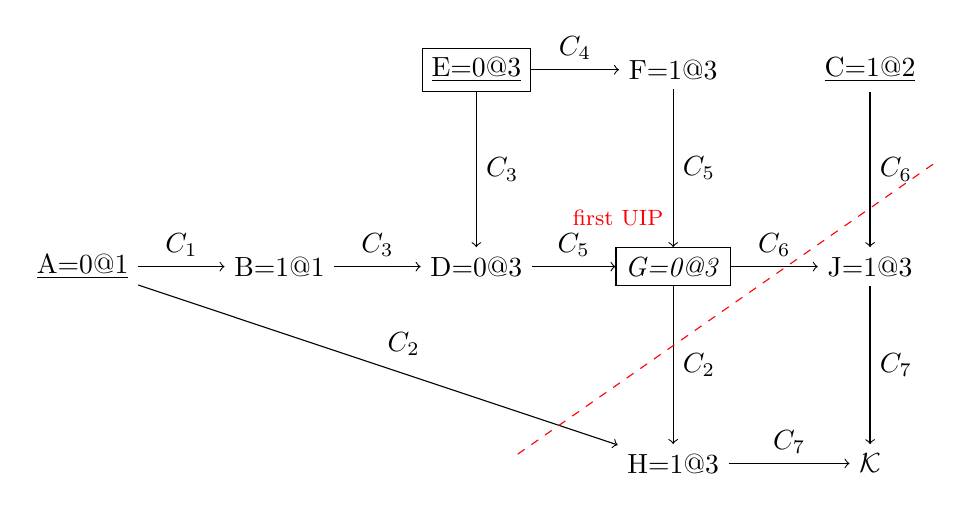
\begin{tikzpicture}[node distance=2.5cm,auto]
	\node (A) {\underline{A=0@1}};
	\node (B) [right of=A] {B=1@1};
	\node (D) [right of=B] {D=0@3};
	%\color{red}
	\node (G) [right of=D, rectangle, draw=black] {\textit{G=0@3}};
	%\color{black}
	\node (H) [below of=G] {H=1@3};
	\node (K) [right of=H] {$\mathcal K$};
	\node (E) [above of=D, rectangle, draw=black] {\underline{E=0@3}};
	\node (F) [right of=E] {F=1@3};
	\node (J) [right of=G] {J=1@3};
	\node (C) [above of=J] {\underline{C=1@2}};
	\path[->] (G) edge node {$C_6$} (J);
	\path[->] (F) edge node {$C_5$} (G);
	\path[->] (C) edge node {$C_6$} (J);
	\path[->] (J) edge node {$C_7$} (K);
	\path[->] (E) edge node {$C_3$} (D);
	\path[->] (E) edge node {$C_4$} (F);

	\path[->] (A) edge node {$C_1$} (B);
	\path[->] (B) edge node {$C_3$} (D);
	\path[->] (D) edge node {$C_5$} (G);
	\path[->] (G) edge node {$C_2$} (H);
	\path[->] (H) edge node {$C_7$} (K);
	\path[->] (A) edge node {$C_2$} (H);

	\node [above,red] at (6.8,0.4) {{\footnotesize \textrm{first UIP}}};
	\draw [red,dashed](10.8,1.3) -- (5.5,-2.4);
	\end{tikzpicture}
	\label{pic:impl_graph}
	\caption{{\protect\small Implication graph with UIPs (nodes with
	rectangles), where the second rectangle node ($G$) with the cursive label
	denotes the \textit{first UIP}.}}
	\end{figure}
	\newline
	%Implication Graph with first UIP (red) and the corresponding cuts (dashed).

	\bigskip

	We have a conflict in $c_{7}$, since $\lnot J$ and $\lnot H$ are not
	satisfied. So we have to resolve and backtrack to the first UIP, which is $%
	G=0@3$.

	Since $c_{2}$, $c_{6}$ and $c_{7}$ are conflict clauses along the out-edges
	and are (the first) on the paths from the first UIP. Hence, the assertion
	clause can be computed, using resolution, as follows:\newline

	% $\tfrac{%
	% \begin{array}{l}
	% c_{2}:A\OR G\OR H \\ 
	% \underline{c_{7}:\lnot J\OR\lnot H}\newline
	% \end{array}%
	% \newline
	% }{c_{8}:A\OR G\OR\lnot J}\tfrac{%
	% \begin{array}{l}
	% c_{6}:\lnot C\OR G\OR J\newline
	% \\ 
	% \underline{c_{8}:A\OR G\OR\lnot J}%
	% \end{array}%
	% \newline
	% }{c_{9}:A\OR\lnot C\OR G}$(after removing the second G with fac.)\newline

	\begin{equation*}
	r_{1}=res(c_{7},c_{2},H)=A\OR G\OR\lnot J\text{\quad and\quad }%
	r_{2}=fac(res(r_{1},c_{6},J))=A\OR\lnot C\OR G.
	\end{equation*}

	The result $r_{2}$ yields the learned clause $c_{8}=(A\OR\lnot C\OR G)$ and
	we backtrack to the highest decision level $DL=3$, i.e. we remove all
	decisions and values at $DL\geq 3$ and change the decision of $E$ to $E=1@3$.

	\medskip

	Thus, we get a new implication graph:\newline

	\begin{figure}[ht]
	\centering
	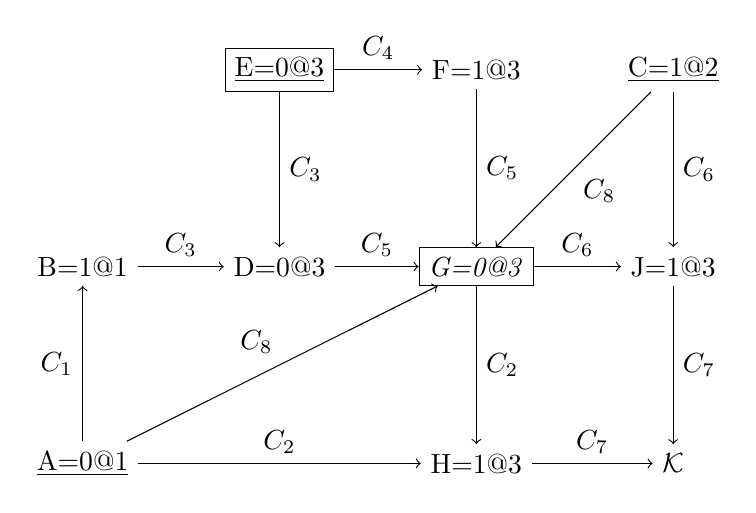
\begin{tikzpicture}[node distance=2.5cm,auto]
	\node (B) {B=1@1};
	\node (A)[below of=B] {\underline{A=0@1}};
	\node (D) [right of=B] {D=0@3};
	\node (G) [right of=D, rectangle, draw=black] {\textit{G=0@3}};
	\node (H) [below of=G] {H=1@3};
	\node (K) [right of=H] {$\mathcal K$};
	\node (E) [above of=D, rectangle, draw=black] {\underline{E=0@3}};
	\node (F) [right of=E] {F=1@3};
	\node (J) [right of=G] {J=1@3};
	\node (C) [above of=J] {\underline{C=1@2}};
	\path[->] (G) edge node {$C_6$} (J);
	\path[->] (F) edge node {$C_5$} (G);
	\path[->] (C) edge node {$C_6$} (J);
	\path[->] (J) edge node {$C_7$} (K);
	\path[->] (E) edge node {$C_3$} (D);
	\path[->] (E) edge node {$C_4$} (F);

	\path[->] (A) edge node {$C_1$} (B);
	\path[->] (B) edge node {$C_3$} (D);
	\path[->] (D) edge node {$C_5$} (G);
	\path[->] (G) edge node {$C_2$} (H);
	\path[->] (H) edge node {$C_7$} (K);
	\path[->] (A) edge node {$C_2$} (H);

	\path[->] (C) edge node {$C_8$} (G);
	\path[->] (A) edge node {$C_8$} (G);
	\end{tikzpicture}
	\label{pic:new_impl_graph}
	\caption{{\protect\small New implication graph with UIPs (nodes with
	rectangles) and the learned clause $c_{8}$.}}
	\end{figure}

	The learned clause $c_{8}$ implies that the node $G$ must be set to $1@3$,
	else $c_{8}$ would be unsatisfied and we get again a new conflict. This
	implies in turn, that the value either in $D$ or in $F$ can be arbitrarily
	chosen. This is also the case for node $J$ and node $H$. One of both nodes
	the value can be arbitrarily chosen and the ohter must be set to $0@3$. By
	setting $F=H=0@3$, we observe that all clauses $c_{i}$, $i\in \{1,\ldots
	,8\} $ are satisfied and obtain a model $M=\{\lnot A,B,C,D,E,F,G,\lnot H,J\}$%
	.

	% \begin{tikzpicture}[node distance=2.5cm,auto]
	% \node (A) {A=0@1};
	% \node (B) [right of=A] {B=1@1};
	% \node (C) [right of=B] {C=1@2};
	% \node (E) [right of=C] {E=1@3};				
	% \path[->] (A) edge node {$c_1$} (B);
	% \end{tikzpicture}
	% \newline
	% \newline
	% The remaining clauses $c_2$, $c_5$, $c_6$ and $c_7$ doesn't contain any
	% rules for the implication graph, so we have to introduce a new decision
	% level $DL 4$ and we can choose the decision for e. g. $G$ as $G = 1@4$:%
	% \newline
	% \bigskip

	% \begin{tikzpicture}[node distance=2.5cm,auto]
	% \node (A) {A=0@1};
	% \node (B) [right of=A] {B=1@1};
	% \node (C) [right of=B] {C=1@2};
	% \node (E) [right of=C] {E=1@3};	
	% \node (G) [right of=E] {G=1@4};			
	% \path[->] (A) edge node {$c_1$} (B);
	% \end{tikzpicture}
	% \newline
	% \newline
	% Again, the remaining clauses $c_5$ and $c_7$ doesn't contain any rules for
	% the implication graph, so we have to introduce a new decision level two
	% times ($DL 5$ and $DL 6$) and we can choose the decisions for e. g. $D$ as $%
	% D = 1@5$ and $H$ as $H = 0@6$:\newline
	% \bigskip

	% \begin{tikzpicture}[node distance=2.5cm,auto]
	% \node (A) {A=0@1};
	% \node (B) [right of=A] {B=1@1};
	% \node (C) [right of=B] {C=1@2};
	% \node (E) [right of=C] {E=1@3};	
	% \node (G) [right of=E] {G=1@4};	
	% \node (D) [below right of=A] {D=1@5};
	% \node (H) [below right of=C] {H=0@6};		
	% \path[->] (A) edge node {$c_1$} (B);
	% \end{tikzpicture}
	% \newline

	% Now we have fulfilled all clauses $c_{i}$, $i\in \{1,...,9\}$ and therefore
	% we can choose any dedcisions for the ramaining values.\newline
	% A valid solution model would be: $\{\lnot A,B,C,D,E,F,G,\lnot H,J\}$

	\bigskip
}

\item Prove that in a conflict graph the first UIP is uniquely defined, i.e.,
  prove that there is exactly one node in the graph which is a first UIP.

 %\solution{
$[p]\sigma = [x:=x+y; \text{ if } x<0 \text{ then } abort \text{ else } while \text{ } x \neq y \text{ } do \text{ }... \text{ } od]\sigma 
\hspace{0.6 cm} \sigma: x \mapsto 1, y \mapsto 1\\
= [\text{if } x<0 \text{ then } abort \text{ else } while \text{ } x \neq y \text{ } do \text{ }... \text{ } od][x:=x+y]\sigma_1
\hspace{1 cm} \sigma_1: x \mapsto [x+y]\sigma = 2\\
\text{} \hspace{12 cm} y \mapsto 1\\
= [\text{if } x<0 \text{ then } abort \text{ else } while \text{ } x \neq y \text{ } do \text{ }... \text{ } od]\sigma_1
\hspace{4 cm} \underbrace{[x<0]\sigma_1=0}_{false}\\
= [\text{while } x \neq y \text{ do } x:=x+1; y:=y+2 \text{ od}]\sigma_1
\hspace{5 cm} \underbrace{[x \neq y]\sigma_1=0}_{true}\\
= [\text{while } x \neq y \text{ do } ... \text{ od}] [x:=x+1;y=y+2]\sigma_1\\
= [\text{while } x \neq y \text{ do } ... \text{ od}] [y:=y+1] [x:=x+1]\sigma_1
\hspace{3 cm} \sigma_2: x \mapsto [x+1]\sigma_1=3\\
\text{} \hspace{11.8 cm} y \mapsto 1\\
= [\text{while } x \neq y \text{ do } ... \text{ od}] [y:=y+2]\sigma_2
\hspace{4.7 cm} \sigma_3: y \mapsto [y+2]\sigma_2=3\\
\text{} \hspace{11.8 cm} x \mapsto 3\\
= [\text{while } x \neq y \text{ do } ... \text{ od}]\sigma_3
\hspace{8 cm} \underbrace{[x \neq y]\sigma_3=0}_{false}\\
= \sigma_3$
%}

\item Let $\mathcal{C}$ be a set of clauses and $G$ a conflict graph with
  respect to $\mathcal{C}$. Prove: if a clause $C_l$ is learned following the
  first-UIP scheme, then $C_l$ is a consequence of $\mathcal{C}$.

  \solution{
  }

\end{enumerate}


%%%%%%%%%%%%%%%%%%%%%%%%%%%%%%%%%%%%%%%%%%%%%%%%%%%%%%%%%%%%%%%%%%%%%%%%%%%%%%

\newpage
\Aufgabe[Sparse Method \hfill \bf (1.5 points)]
Apply the Sparse Method including preprocessing on the formula $\varphi^E$
below to obtain a propositional formula.
\begin{displaymath}
  (x_1 \neq x_2 \lor x_2=x_3 ) \land \big[ (x_2 \neq x_4 \land x_3=x_4
  \land x_4=x_5)
  \lor (x_6 \neq x_5 \land x_6=x_7 \land x_7=x_3)\big]
\end{displaymath}

















\subsection{solution}

test



%%%%%%%%%%%%%%%%%%%%%%%%%%%%%%%%%%%%%%%%%%%%%%%%%%%%%%%%%%%%%%%%%%%%%%%%%%%%%%

\newpage
\Aufgabe[Ackermann's Reduction \hfill \bf (1 point)]
Apply Ackermann's reduction on the following EUF-formula $\varphi$ to obtain
an EU formula:
\begin{displaymath}
  f\left(f\left(g\left(a\right),b\right),a\right) = f(g(a),b) \rightarrow \big[ f(x,y) = g(f(g(a),b)) \land
  g(f(a,y))=d \big]
\end{displaymath}

\subsection{solution}

test



\end{document}
